\section{Fizyka statystyczna i optymalizacja - analogie}

%%%%%%%%%%%%%%%% 
	\begin{frame}{Fizyka statystyczna i optymalizacja - analogie}
		\begin{block}{Fizyka statystyczna}
				uśrednione wartości dla zespołów o dużej ilości molekuł	
		\end{block}
		
		
		\begin{table}[]
		\centering
		\begin{tabular}{|l|l|}
		\hline
		\textbf{Mechanika statystyczna}                                                                                                 & \textbf{Optymalizacja}                                                                  \\ \hline
		wiele oddziałujących molekuł                                                                                                    & wiele parametrów                                                                        \\ \hline
		układ, zbiór położeń molekuł                                                                                                    & konfiguracja                                                                            \\ \hline
		\begin{tabular}[c]{@{}l@{}}schłodzenie do stabilnego stanu \\ niskoenergetycznego\end{tabular}                                  & \begin{tabular}[c]{@{}l@{}}znalezienie konfiguracji \\ prawie optymalnej\end{tabular}   \\ \hline
		temperatura                                                                                                                     & \begin{tabular}[c]{@{}l@{}}parametr sterujący \\ przebiegiem optymalizacji\end{tabular} \\ \hline
		hamiltonian (operator energii) \\                                                                             & funkcja celu                                                                            \\ \hline
		\begin{tabular}[c]{@{}l@{}}w hamiltonianie człony \\
		wynikające z róznych oddziaływań
		\end{tabular} & \begin{tabular}[c]{@{}l@{}}współzawodniczące człony \\ w funkcji celu\end{tabular}      \\ \hline
		\end{tabular}
		\end{table}

	\end{frame}
	\begin{frame}{Przykład: problem Max-Cut}
 \begin{figure}
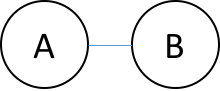
\includegraphics[scale=0.3]{img/18/barbell.png}
%\caption{Graph to cut}
\end{figure} 
\begin{figure}
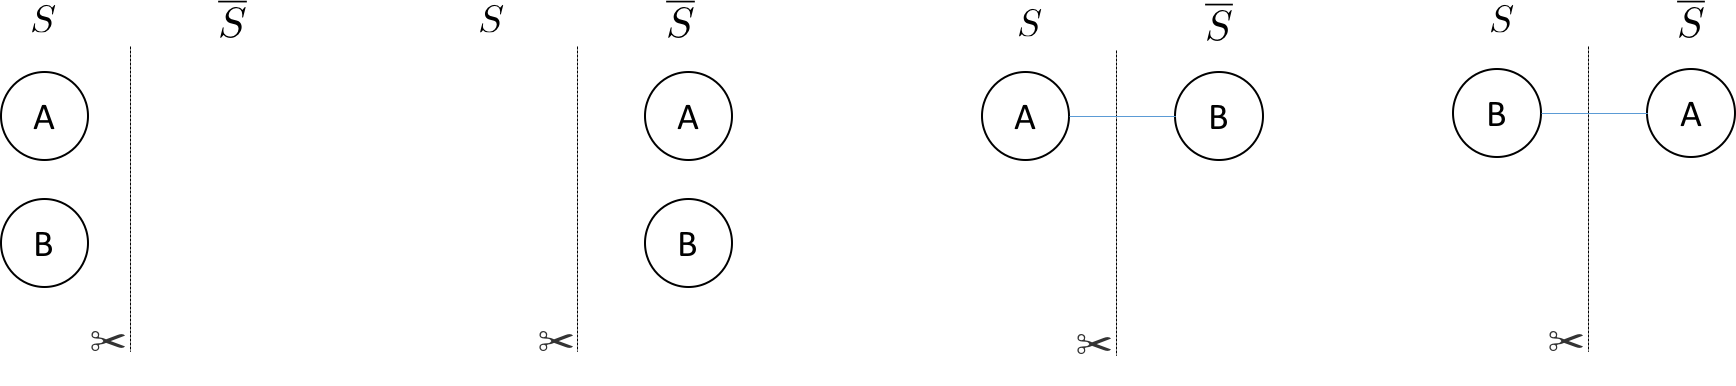
\includegraphics[scale=0.18]{img/18/partition_barbell.png}
%\caption{Cutting possibilities}
\end{figure} 
Funkcja kosztu:
    \begin{itemize}
        \item[] $g(x_1, x_2)=x_1+x_2-2x_1 x_2$, $x_1,x_2 \in\{0,1\}$
        \item[] $g(00)=0$ $g(11)=0$
        \item[] $g(01)=1$ $g(10)=1$
    \end{itemize}
    \\
    \small{source: https://grove-docs.readthedocs.io/en/latest/qaoa.html}
\end{frame}

\begin{frame}{Hamiltonian dla MaxCut}
Mamy efektywną symulację dla modelu Isinga:
\url{http://www.bdhammel.com/ising-model/}
  \url{https://stanford.edu/~jeffjar/statmech/intro4.html} \\
  Funkcja kosztu naszego problemu:
    \begin{itemize}
        \item[] $g(x_1, x_2)=x_1+x_2-2x_1 x_2$, $x_1,x_2 \in\{0,1\}$
       \end{itemize}
W modelu Isinga
       \begin{itemize}
           \item  x=0 - spin do góry (z=1)
           \item  x=1 - spin w dół (z=-1)
       \end{itemize}
    
Funkcja energii zależna od konfiguracji\_spinów     
       \begin{itemize}
        \item[] $x\rightarrow \frac{1}{2}(1-z)$  
        \item[] $g(z_1,z_2)=\frac{1}{2}(1-z_1z_2)$ $z_1,z_2 \in\{-1,1\}$
   \end{itemize}     
\end{frame}
\begin{frame}{Model Isinga}
$$ H_{\text{maxcut}}=\frac{1}{2}  - \frac{1}{2} \sum_{<ij>} {z_{i}} {z_{j}}$$

$$ H_{\text{Ising}}=- \sum_{i} h_i z_i - \sum_{<ij>} J_{i,j} z_{i} z_{j}
$$
$$H_{\text{maxcut}}=\frac{1}{2} - \frac{1}{2} H_{\text{Ising}}$$
dla $h=0$, $J=-1$\\

\end{frame}%\begin{frame}{Notacja Diraca, iloczyn tensorowy}
 %  $$\ket{0}=\begin{bmatrix}1\\0
  %      \end{bmatrix}
   %     \ket{1}=\begin{bmatrix}0\\1
    %    \end{bmatrix}$$ 
%        $$\ket{00}=\begin{bmatrix}1\\0\\0\\0
%        \end{bmatrix}
%        \ket{01}=\begin{bmatrix}0\\1\\0\\0
%        \end{bmatrix}
%        \ket{10}=\begin{bmatrix}0\\0\\1\\0
%        \end{bmatrix}
%        \ket{11}=\begin{bmatrix}0\\0\\0\\1
%        \end{bmatrix}$$ 
%        $$\ket{01}=\ket{0}\otimes\ket{1}=
%        \begin{bmatrix}1\\0
%        \end{bmatrix}\otimes
%\begin{bmatrix}0\\1
%        \end{bmatrix}=
%        \begin{bmatrix}1\cdot0\\1\cdot1\\0\cdot0%\\0\cdot1
%        \end{bmatrix}=\begin{bmatrix}0\\1\\0\\0
%        \end{bmatrix}$$
%        
%\end{frame}
%\begin{frame}{Hamiltonian dla MaxCut}
%Funkcja kosztu:
 %   \begin{itemize}
 %       \item[] $g(x_1, x_2)=x_1+x_2-2x_1 x_2$, $x_1,x_2 \in\{0,1\}$
  %      \item[] $x\rightarrow \frac{1}{2}(1-z)$  
   %     \item[] $g(z_1,z_2)=\frac{1}{2}(1-z_1z_2)$ $z_1,z_2 \in\{-1,1\}$
    %    \item[]
     %   $\sigma_z=\begin{pmatrix}  
%    1 &0\\
 %    0 & -1\\
  %  \end{pmatrix}$
   %     \item[] $\sigma_z\ket{0}=\ket{0}, \lambda=1$
    %    \item[] $\sigma_z\ket{1}=-\ket{1}, %\lambda=-1$
     %   \item[] aby zbudować Hamiltonian: $z\rightarrow \sigma_z$
      %  \item[] $H_{i,j}=\frac{1}{2}(I-{\sigma_z}^i\otimes {\sigma_z}^j)=\begin{pmatrix}  
    %0 &0&0&0\\
    % 0 &1&0&0\\
     % 0 &0&1&0\\
     %  0 &0&0&0
    %\end{pmatrix} \begin{matrix}
    %\ket{00}\\
    % \ket{01}\\
    %  \ket{10}\\
    %   \ket{11}\\
    %\end{matrix}$
     %   \item[]Wartości włąsne
      %  \begin{itemize}
       %     \item $0$ dla $\ket{00}$ i %$\ket{11}$ ; $g(00)=0$ $g(11)=0$
    %         \item $1$ dla $\ket{01}$ i %$\ket{10}$ ; $g(01)=1$ $g(10)=1$
    %    \end{itemize}
    %\end{itemize}
    %\\
    %\small{source: %https://grove-docs.readthedocs.io/en/latest/qaoa.html}
%\end{frame}
%%$$ H_{\text{maxcut}}=\frac{1}{2} I - \frac{1}{2} \sum_{<ij>} {\sigma_{z}_{(i)}} {\sigma_{z}_{(j)}}$$

%$$ H_{\text{Ising}}=- \sum_{i} h_i %{\sigma_{z}_{(i)}} - \sum_{<ij>} J_{i,j} %{\sigma_{z}_{(i)}} {\sigma_{z}_{(j)}}
%$$
%$$H_{\text{maxcut}}=\frac{1}{2} - \frac{1}{2} H_{\text{Ising}}$$
%dla $h=0$, $J=-1$\\
%\url{http://www.bdhammel.com/ising-model/}
%  \url{https://stanford.edu/~jeffjar/statmech/intro4.html} 
%\end{frame}
